\section{Graphing functions}
\label{sec:graphing}

Among the most common types of figures for \TeX{} users are those which
are the graphs of functions of a single variable.  Hobby recognized this
and constructed a package to accomplish this task.  It is invoked by

\begin{lstlisting}[xleftmargin=80bp]
input graph;
\end{lstlisting}

\MP{} has the ability to construct data (i.e., ordered pairs) for
graphing simple functions.  However, for more complicated functions, the
data should probably be constructed using external programs such as
\acro{MATLAB} (or Octave), Maple, Mathematica, Gnuplot, et. al.

A typical data file, say \textattachfile[color={0 0
  0},mimetype={text/plain}]{data.d}{\texttt{data.d}}, to be used with
the \texttt{graph} package may have contents

\lstinputlisting[xleftmargin=77bp]{data.d}

This data represents the graph of $f(x)=\sqrt{x}$ for six equally spaced
points in $[0,1]$.  To graph this data, the size of the graph must first
be decided.  Choosing a width of $144\mathrm{\ bp}$ and a height of
$89\mathrm{\ bp}$, a minimally controlled plot (as in Figure
\ref{fig:data}) of this data can be generated by

\begin{lstlisting}[xleftmargin=38bp]
draw begingraph(144bp,89bp);
   gdraw "data.d";
endgraph;
\end{lstlisting}

The \texttt{graph} package provides many commands used to customize
generated graphs, and these commands are fully documented in the manual
\cite{hobby:graph} for the \texttt{graph} package.

\begin{figure}[hptb]
   \begin{center}
     \textattachfile[color={0 0 0},mimetype={text/plain}]{data.mp}{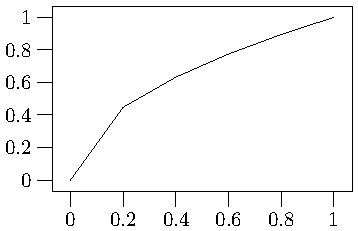
\includegraphics{data.mps}}
   \end{center}
   \caption{$f(x)=\sqrt{x}$ using the \texttt{graph} package}
   \label{fig:data}
\end{figure}
